\documentclass[tikz,border=2pt]{standalone}
\usepackage{amsmath}
\usepackage{pgfplots}
\pgfplotsset{compat=1.18}

\begin{document}
% A sequence is a list indexed by n = 1, 2, 3, ...: here a_n = (-1)^n/n plotted against its index.
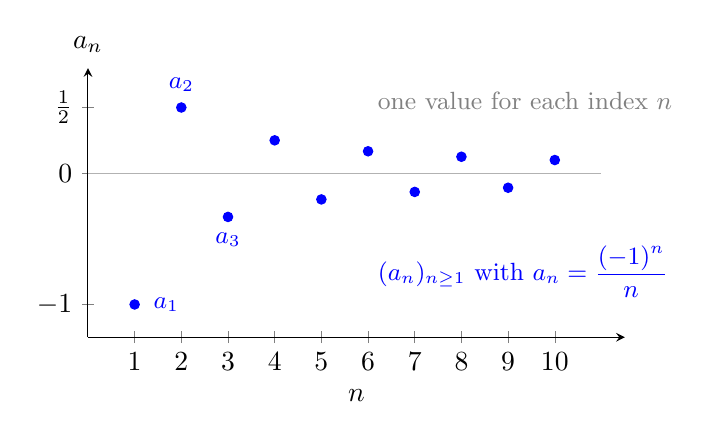
\begin{tikzpicture}
	\begin{axis}[
		axis lines=left,
		xmin=0, xmax=11.5,
		ymin=-1.25, ymax=0.8,
		xtick={1,...,10}, ytick={-1,0,0.5}, yticklabels={$-1$,$0$,$\tfrac12$},
		xlabel={$n$}, ylabel={$a_n$}, ylabel style={rotate=-90, anchor=south, at={(axis description cs:0,1.02)}},
		clip=false,
		width=8.4cm, height=5cm
		]
		\draw[gray!60] (axis cs:0,0) -- (axis cs:11,0);
		\addplot[only marks, mark=*, mark size=1.7pt, blue, samples at={1,...,10}] {(-1)^x/x};
		\node[blue, anchor=west, font=\small] at (axis cs:1.2,-1.0) {$a_1$};
		\node[blue, anchor=south, font=\small] at (axis cs:2,0.55) {$a_2$};
		\node[blue, anchor=north, font=\small] at (axis cs:3,-0.38) {$a_3$};
		\node[blue, anchor=west, font=\small] at (axis cs:6,-0.75) {$(a_n)_{n\ge1}$ with $a_n=\dfrac{(-1)^n}{n}$};
		\node[gray, anchor=west, font=\small] at (axis cs:6,0.55) {one value for each index $n$};
	\end{axis}
\end{tikzpicture}
\end{document}
